\documentclass[UTF8]{article}
\usepackage{graphicx}
\usepackage{subfigure}
\usepackage{amsmath}
\usepackage{makecell}
\usepackage[utf8]{inputenc}
\usepackage[space]{ctex} %中文包
\usepackage{listings} %放代码
\usepackage{xcolor} %代码着色宏包
\usepackage{CJK} %显示中文宏包
\usepackage{float}
\usepackage{makecell}
\usepackage{diagbox}
\usepackage{bm}
\usepackage{ulem} 
\usepackage{amssymb}
\usepackage{soul}
\usepackage{color}
\usepackage{geometry}
\usepackage{fancybox} %花里胡哨的盒子
\usepackage{xhfill} %填充包, 可画分割线 https://www.latexstudio.net/archives/8245
\usepackage{multicol} %多栏包
\usepackage{enumerate} %可以方便地自定义枚举标题
\usepackage{multirow} %表格中多行单元格合并
\usepackage{wasysym} %可以使用wasysym里的一堆奇奇怪怪的符号
\usepackage{tikz}
\usepackage{tikZ-timing} % 时序图支持
\usepackage{pgfplots} % http://pgfplots.sourceforge.net/gallery.html
\usetikzlibrary{pgfplots.patchplots} % 拟合支持
\usetikzlibrary{shadows} % 阴影支持

\geometry{left = 1.5cm, right = 1.5cm, top=1.5cm, bottom=2cm}

\definecolor{mygreen}{rgb}{0,0.6,0}
\definecolor{mygray}{rgb}{0.5,0.5,0.5}
\definecolor{mymauve}{rgb}{0.58,0,0.82}
\lstset{
	backgroundcolor=\color{white}, 
	%\tiny < \scriptsize < \footnotesize < \small < \normalsize < \large < \Large < \LARGE < \huge < \Huge
	basicstyle = \footnotesize,       
	breakatwhitespace = false,        
	breaklines = true,                 
	captionpos = b,                    
	commentstyle = \color{mygreen}\bfseries,
	extendedchars = false,
	frame = shadowbox, 
	framerule=0.5pt,
	keepspaces=true,
	keywordstyle=\color{blue}\bfseries, % keyword style
	language = C++,                     % the language of code
	otherkeywords={string}, 
	numbers=left, 
	numbersep=5pt,
	numberstyle=\tiny\color{mygray},
	rulecolor=\color{black},         
	showspaces=false,  
	showstringspaces=false, 
	showtabs=false,    
	stepnumber=1,         
	stringstyle=\color{mymauve},        % string literal style
	tabsize=4,          
	title=\lstname           
}

%\sum\nolimits_{j=1}^{M}   上下标位于求和符号的水平右端,
%\sum\limits_{j=1}^{M}   上下标位于求和符号的上下处,
%\sum_{j=1}^{M}  对上下标位置没有设定,会随公式所处环境自动调整。

%%%%%%%%%%%%%画图包%%%%%%%%%%%%%
\usepackage{tikz}
%%%%%%%%%%%%%好看的矩形%%%%%%%%%%%%%
\tikzset{
  rect1/.style = {
    shape = rectangle,% 指定样式
    minimum height=2cm,% 最小高度
    minimum width=4cm,% 最小宽度
    align = center,% 文字居中
    drop shadow,% 阴影
  }
}
%%%%%%%%%%%%%画图背景包%%%%%%%%%%%%%
\usetikzlibrary{backgrounds}

%%%%%%%%%%%%%在tikz中画一个顶点%%%%%%%%%%%%%
%%%%%%%%%%%%%#1:node名称%%%%%%%%%%%%%
%%%%%%%%%%%%%#2:位置%%%%%%%%%%%%%
%%%%%%%%%%%%%#3:标签%%%%%%%%%%%%%
\newcommand{\newVertex}[3]{\node[circle, draw=black, line width=1pt, scale=0.8] (#1) at #2{#3}}
%%%%%%%%%%%%%在tikz中画一条边%%%%%%%%%%%%%
\newcommand{\newEdge}[2]{\draw [black,very thick](#1)--(#2)}
%%%%%%%%%%%%%在tikz中放一个标签%%%%%%%%%%%%%
%%%%%%%%%%%%%#1:名称%%%%%%%%%%%%%
%%%%%%%%%%%%%#2:位置%%%%%%%%%%%%%
%%%%%%%%%%%%%#3:标签内容%%%%%%%%%%%%%
\newcommand{\newLabel}[3]{\node[line width=1pt] (#1) at #2{#3}}

%%%%%%%%%%%%%强制跳过一行%%%%%%%%%%%%%
\newcommand{\jumpLine} {\hspace*{\fill} \par}
%%%%%%%%%%%%%关键点指令,可用itemise替代%%%%%%%%%%%%%
\newcommand{\average}[1]{\left\langle #1\right\rangle }
%%%%%%%%%%%%%表格内嵌套表格%%%%%%%%%%%%%
\newcommand{\keypoint}[2]{$\bullet$\textbf{#1}\quad#2\par}
%%%%%%%%%%%%%<T>平均值表示%%%%%%%%%%%%%
\newcommand{\tabincell}[2]{\begin{tabular}{@{}#1@{}}#2\end{tabular}}%放在导言区
%%%%%%%%%%%%%大黑点item头%%%%%%%%%%%%%
\newcommand{\itemblt}{\item[$\bullet$]}
%%%%%%%%%%%%%大圈item头%%%%%%%%%%%%%
\newcommand{\itemc}{\item[$\circ$]}
%%%%%%%%%%%%%大星星item头%%%%%%%%%%%%%
\newcommand{\itembs}{\item[$\bigstar$]}
%%%%%%%%%%%%%右▷item头%%%%%%%%%%%%%
\newcommand{\itemrhd}{\item[$\rhd$]}
%%%%%%%%%%%%%定义为%%%%%%%%%%%%%
\newcommand{\defas}{=_{df}}
%%%%%%%%%%%%%蕴含%%%%%%%%%%%%%
\newcommand{\imp}{\rightarrow}
%%%%%%%%%%%%%偏导%%%%%%%%%%%%%
\newcommand{\partialx}[2]{\frac{\partial #1}{\partial #2}}

%%%%%%%%%%%%%双线分割线%%%%%%%%%%%%%
\newcommand*{\doublerule}{\hrule width \hsize height 1pt \kern 0.5mm \hrule width \hsize height 2pt}
%%%%%%%%%%%%%双线中间可加东西的分割线%%%%%%%%%%%%%
\newcommand\doublerulefill{\leavevmode\leaders\vbox{\hrule width .1pt\kern1pt\hrule}\hfill\kern0pt }
%%%%%%%%%%%%%左大括号%%%%%%%%%%%%%
\newcommand{\leftbig}[1]{\left\{\begin{array}{l}#1\end{array}\right.}
%%%%%%%%%%%%%矩阵%%%%%%%%%%%%%
\newcommand{\mat}[2]{\left[\begin{array}{#1}#2\end{array}\right]}
%%%%%%%%%%%%%可换行圆角文本框%%%%%%%%%%%%%
\newcommand{\ovalboxn}[1]{\ovalbox{\tabincell{l}{#1}}}
%%%%%%%%%%%%%背景黄色%%%%%%%%%%%%%
\newcommand{\highlight}[1]{\text{\colorbox{yellow}{$#1$}}}
\newcommand{\colorboxm}[2]{\text{\colorbox{#1}{$#2$}}}
%%%%%%%%%%%%%背景黄色%%%%%%%%%%%%%
\newcommand{\highlightnew}[2][]{\tcbhighmath[size=minimal,colframe=yellow,colback=yellow,#1]{#2}}
%%%%%%%%%%%%%设置section的counter, 使从0开始%%%%%%%%%%%%%
\setcounter{section}{0}

\begin{document}
\section{数学基础}
https://www.cnblogs.com/pinard/archive/2004/01/13/10791506.html
\subsection{矩阵}
\subsubsection{迹相关性质}
\begin{itemize}
\item 转置不变性: $tr(A^T)=tr(A)$
\item 迹的循环相等性: $tr(ABC)=tr(BCA)=tr(CAB)$
\item 加减分配: $tr(X\pm Y)=tr(X)\pm tr(Y)$
\item 乘法和迹交换: $tr((A\odot B)^TC)=tr(A^T(B\odot C))$
\end{itemize}

\subsection{矩阵导数}
\subsubsection{导数布局}
\begin{tabular}{|c|c|c|c|}
\hline
行头对列头求导 & 标量$y$ & m维向量$\bm{y}$ & $p\times q$维矩阵$\bm{Y}$ \\
\hline
标量$x$ & $1\times1$ & $m\times 1$ & $\partialx{\bm{Y}}{x}$, $p\times q$ \\
\hline
n维向量$\bm{x}$ & $\partialx{y}{\bm{x}}$, $n\times 1$ & $n\times m$ &  \\
\hline
$r\times s$维矩阵$\bm{X}$ & $\partialx{y}{\bm{X}}$, $r\times s$ &  &  \\
\hline
\end{tabular}
\subsubsection{标量对张量求导}
标量值函数的矩阵微分定义为:
$$\highlight{df=\sum\limits_{i,j}\partialx{f}{X_{ij}}dX_{ij}=tr((\partialx{f}{X})^TdX)=tr((\partialx{f}{X})dX^T)}$$
并且具有如下常用性质:
\begin{enumerate}
\item $d(X\pm Y)=dX\pm dY$, $d(XY)=(dX)Y+X(dY)$, $d(X\odot Y)=(dX)\odot Y+X\odot (dY)$
\item $d(X^T)=(dX)^T$, $d(tr(X))=tr(dX)$
\item $dX^{-1}=-X^{-1}(dX)X^{-1}$
\item $d|X|=|X|tr(X^{-1}dX)$
\item 逐元素求导: $d\sigma(X)=\sigma'(X)\odot dX$
\end{enumerate}
\ovalboxn{
例题1. 求$\partialx{tr(ABA^T)}{A}$\\
$d(tr(ABA^T))=tr((dA)BA^T+AB(dA^T))=tr(AB^T(dA)^T)+tr(AB(dA)^T)=tr(A(B^T+B)(dA)^T)$\\
故有$\partialx{tr(ABA^T)}{A}=A(B^T+B)$
}\\
\ovalboxn{
例题2. $y=\bm{a}^Texp(X\bm{b})$, 求$\partialx{y}{X}$\\
$dy=tr(dy)=tr(\bm{a}^Tdexp(X\bm{b}))=tr(\bm{a}^Texp(X\bm{b})\odot d(X\bm{b}))=tr((\bm{a}\odot exp(X\bm{b}))^T d(X\bm{b}))=tr(b(a\odot exp(X\bm{b}))^TdX)$\\
故$\partialx{y}{X}=(a\odot exp(X\bm{b}))b^T$
}
\subsubsection{链式法则}
\begin{itemize}
\item 比如$\partialx{\bm{y}}{\bm{x}}$, 本质上就是对中间变量的每个分量对$\bm{x}$求导乘上$\bm{y}$对中间变量的每个分量求导, 然后求和.
\end{itemize}
\subsubsection{对向量求导链式法则}
\begin{itemize}
\item 向量对向量的链式法则: $$\partialx{\bm{z}}{\bm{x}}=\partialx{\bm{z}}{\bm{y}}\partialx{\bm{y}}{\bm{x}}$$
\item 标量对向量的链式法则: $$\partialx{z}{\bm{x}}=\partialx{\bm{y}}{\bm{x}}\partialx{z}{\bm{y}},\qquad((len(\bm{x}), len(\bm{y}))\cdot (len(\bm{y}), 1))$$
$$\partialx{z}{\bm{x}}=(\partialx{\bm{y_n}}{\bm{y_{n-1}}}\partialx{\bm{y_{n-1}}}{\bm{y_{n-2}}}\cdots\partialx{\bm{y_2}}{\bm{y_{1}}})\partialx{z}{\bm{y_n}},\qquad((len(\bm{y_n}), len(\bm{y_1}))\cdot (len(\bm{y}), 1))$$
\ovalboxn{例题1. 最小二乘法损失函数的求导, 即求$\partialx{l}{\theta}$, 这里$l=(X\bm{\theta}-\bm{y})^T(X\bm{\theta}-\bm{y})$\\
令$\bm{z}=X\bm{\theta}-\bm{y}$\\
则$\partialx{l}{\bm{\theta}}=(\partialx{\bm{z}}{\bm{\theta}})\partialx{l}{\bm{z}}=X^T\partialx{\bm{z}^T\bm{z}}{\bm{z}}$\\
而$tr(d(\bm{z}^T\bm{z}))=tr(\bm{z}^T(d\bm{z})+(d\bm{z}^T)\bm{z})=tr(\bm{z}^T(d\bm{z})+(\bm{z}d\bm{z}^T))=tr(2\bm{z})$\\
所以$\partialx{l}{\bm{\theta}}=X^T2\bm{z}=2X^T(X\bm{\theta}-\bm{y})$}
\end{itemize}
\subsubsection{特殊求导}
\begin{itemize}
\item 梯度: $\nabla f(\bm{x})_i=\partialx{f(\bm{x})}{x_i}$
\item 海森矩阵: $\nabla^2 f(\bm{x})_{ij}=\frac{\partial^2f(\bm{x})}{\partial x_i\partial x_j}$
\item Frobenius范数求导: $\partialx{\|A\|_F^2}{A}=\partialx{A^TA}{A}=2A$
\end{itemize}

\subsection{矩阵分解}
\subsubsection{特征值分解}
\begin{itemize}
\item 特征方程: $A\bm{v}=\lambda\bm{v}$
\item 特征值分解: $A=Vdiag(\bm{\lambda})V^{-1}$, $V$的每一列为特征向量$\bm{v_i}$
\item 特征值为正(非负)的矩阵为\textbf{正定(半正定)矩阵}
\item 可特征值分解(可对角化)的充分条件: 实对称矩阵
\item 手算分解方法: 求出特征向量就行了.
\end{itemize}
\subsubsection{奇异值分解}
\begin{itemize}
\item 设矩阵$A\in C^{m\times n}$, $A^TA\bm{v}=\lambda\bm{v}$, \\
	令$A\bm{v}=\sigma\bm{u}$, 则
	\begin{itemize}
	\item 两边同乘$AA^T$得到, $AA^T\bm{u}=\frac{\lambda}{\sigma}A\bm{v}=\lambda\bm{u}$, $\bm{u}$对应$AA^T$的特征值为$\lambda$的特征向量
	\item 两边同左乘$\bm{u}^T$得到, $\bm{u}^TA\bm{v}=\sigma$
	\item 两边同左乘$\bm{v}^TA^T$得到, $\frac{\lambda}{\sigma}=\bm{v}^TA^T\bm{u}=\bm{u}^TA\bm{v}$
	\end{itemize}
	因此$\lambda=\sigma^2$\\
	写成矩阵形式, 有$AV=U\Sigma$即$A=U\Sigma V^T$, 其中$U\in C^{m\times m}$, 为$AA^T$的特征向量构成矩阵; $\Sigma\in C^{m\times n}$; $V\in C^{n\times n}$, 为$A^TA$的特征向量构成矩阵
\item 任意矩阵都可以作奇异值分解
\item 截断奇异值分解: $A\approx U_k\Sigma_kV_k^T$, $U_k\in C^{m\times k}$即取前k列; $\Sigma_k\in C^{k\times k}$; $V_k\in C^{n\times k}$, 即取前k行
\end{itemize}

\subsection{概率分布}
\begin{itemize}
\item 多元正态分布
	\begin{itemize}
	\item $\mathcal{N}(\bm{x}; \bm{\mu},\Sigma)=\frac{1}{\sqrt{(2\pi)^ndet(\Sigma)}}=exp\left(-\frac{1}{2}(\bm{x}-\bm{\mu})^T\Sigma^{-1}(\bm{x}-\bm{\mu})\right)$
	\item $\mathcal{N}(\bm{x}; \bm{\mu},\bm{\beta}^{-1})=\sqrt{\frac{det(\bm{\beta})}{(2\pi)^n}}=exp\left(-\frac{1}{2}(\bm{x}-\bm{\mu})^T\bm{\beta}(\bm{x}-\bm{\mu})\right)$
	\end{itemize}
\item 贝塔分布
	\begin{itemize}
	\item 概率密度函数: $$Beta(\mu|a,b)=\frac{\Gamma(a+b)}{\Gamma(a)\Gamma(b)}\mu^{a-1}(1-\mu)^{b-1}$$
	\item $E[\mu]=\frac{a}{a+b}$
	\item $Var[\mu]=\frac{ab}{(a+b)^2(a+b+1)}$
	\end{itemize}
\item 狄利克雷分布(是贝塔分布的多元扩展)
	\begin{itemize}
	\item 多个连续变量$\mu_i\in[0,1]$的分布, 满足$\sum\mu_i=1$
	\item $Dir(\bm{\mu}|\bm{\alpha})=\frac{\Gamma(\sum_i\alpha_i)}{\Pi_i\alpha_i}\Pi_i\mu_i^{\alpha_i-1}$
	\item $E[\mu_i]=\frac{\alpha_i}{\sum_i\alpha_i}$
	\end{itemize}
\item 伽马分布($\tau>0$)
	\begin{itemize}
	\item $Gam(\tau|a,b)=\frac{1}{\Gamma(a)}b^a\tau^{a-1}e^{-b\tau}$
	\item $E[\tau]=\frac{a}{b}$
	\item $Var[\tau]=\frac{a}{b^2}$
	\end{itemize}
\end{itemize}

\subsection{K-L散度}
\begin{itemize}
\item 衡量两个分布的差异
	\begin{itemize}
	\item K-L散度定义: $$D_{KL}(P\|Q)=E_{X\sim P}\left[log\frac{P(x)}{Q(x)}\right]$$
	即$$D_{KL}(P\|Q)=\colorboxm{cyan}{E_{X\sim P}logP(x)} - \colorboxm{lime}{E_{X\sim P}{Q(x)}}$$
	$\colorboxm{cyan}{E_{X\sim P}logP(x)}$为P的熵, $\colorboxm{lime}{E_{X\sim P}{Q(x)}}$为P和Q的交叉熵
	\item 非负, P=Q时为0
	\item $D_{KL}(P\|Q)\not=D_{KL}(Q\|P)$, 但理论上最小值都是P=Q
	\end{itemize}
\end{itemize}

\subsection{优化}
\begin{itemize}
\item 标准优化问题: $$\min\limits_{\bm{x}}f(\bm{x})
s.t.\left\{\begin{array}{l}g_i(\bm{x})\le0,i=1,2,\cdots,m\\h_j(\bm{x})=0,j=1,2,\cdots,n\end{array}\right.$$
\item 凸函数
	\begin{itemize}
	\item 定义(零阶条件): 对于$f:\mathbb{R}^n\mapsto \mathbb{R}$, 若$\forall t\in[0,1],f(t\bm{x}+(1-t)\bm{y})\le tf(\bm{x})+(1-t)f(\bm{y})$, 则$f$为凸函数
	\item 一阶条件: $f(\bm{y})\ge f(\bm{x})+\nabla f(\bm{x})^T(\bm{y}-\bm{x})$
	\item 二阶条件: $\nabla^2f(\bm{x})\ge 0$, 即海森矩阵半正定
	\end{itemize}
\item 凸优化问题: $$\min\limits_{\bm{x}}f(\bm{x}) s.t.\left\{\begin{array}{l}g_i(\bm{x})\le0,i=1,2,\cdots,m\\\bm{a}_i^T\bm{x}=b,j=1,2,\cdots,n\end{array}\right.$$
\item 无约束优化: 梯度下降: $x_{t+1}\leftarrow x_t-\alpha\nabla f(x_t)$
\item 有约束优化: 拉格朗日乘子法
	\begin{itemize}
	\item 拉格朗日函数: $L(\bm{x},\bm{u},\bm{v})=f(\bm{x})+\sum\limits_iu_ig_i(\bm{x})+\sum\limits_jv_jh_j(\bm{x})$, 其中$u_i\ge0$
	\item $\forall \bm{u}\ge 0,\bm{v}$和可行解$\bm{x}$, 有$$L(\bm{x},\bm{u},\bm{v})\le f(\bm{x})$$
	\item 对偶问题: $$\max\limits_{\bm{u},\bm{v}}g(\bm{u},\bm{v}),\ s.t.\ \bm{u}\ge0$$
	其中$g(\bm{u},\bm{v})=\min\limits_{\bm{x}}L(\bm{x},\bm{u},\bm{v})$
	\item 弱对偶性: 设可行解集$C$, 原问题最优解$f^*$, 则$$f^*\ge\min\limits_{\bm{x}\in C}L(\bm{x},\bm{u},\bm{v})\ge\min\limits_{\bm{x}}L(\bm{x},\bm{u},\bm{v})=g(\bm{u},\bm{v})$$
	从而得到$$f^*\ge g^*=\max\limits_{\bm{u},\bm{v}}g(\bm{u},\bm{v})$$
	\end{itemize}
\end{itemize}

\newpage
\section{模型评估与选择}
\subsection{误差与过/欠拟合}
\begin{itemize}
\item 误差: 预测与实际之差异
\item 训练误差/经验误差: 在训练集上的误差
\item 泛化误差: 在新样本上的误差
\item 过拟合/欠拟合
\end{itemize}
\subsection{评估方法}
\subsubsection{数据集划分}
\begin{itemize}
\item 留出法: 
	\begin{itemize}
	\item 注意分层采样以保留比例
	\item 一般采用若干次随即划分取平均值作为留出法的评估结果.
	\item 一般将$2/3\sim4/5$的样本用于训练
	\end{itemize}
\item k折交叉验证法
	\begin{itemize}
	\item 最常用k=10
	\item 当k=m(即数据集D中样本数)时, 称为留一法. 准确(未必)但开销大.
	\end{itemize}
	\begin{minipage}{0.5\linewidth}
	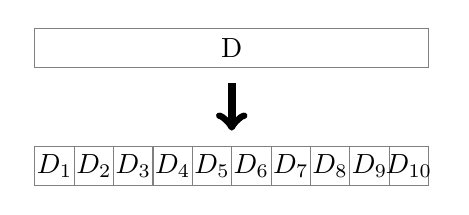
\begin{tikzpicture}
	\draw[color=gray] (0, 1.5) rectangle (5, 2); \node at (2.5, 1.75) {D};
	\draw[->, line width=1mm] (2.5,1.3)--(2.5,0.7);
	\draw[step=0.5cm,color=gray] (0, 0) grid (5,0.5);
	\foreach \i in {1,...,10}
	{
		\pgfmathsetmacro{\xi}{\i/2-0.25};
		\node at (\xi,0.25) {$D_{\i}$};
	}
	\end{tikzpicture}
	\end{minipage}
	\begin{minipage}{0.5\linewidth}
	\begin{tikzpicture}
	\node at (2.25, 0.5) {训练集};
	\node[color=orange] at (5.25, 0.5) {测试集};
	\draw[step=0.5cm,color=gray] (0, -0.5) grid (4.5,0);
	\foreach \i in {1,...,9}
	{
		\pgfmathsetmacro{\xi}{\i/2-0.25};
		\node at (\xi,-0.25) {$D_{\i}$};
	}
	\draw[color=orange] (5, -0.5) rectangle (5.5, 0); \node at (5.25, -0.25) {$D_{10}$};
	
	\draw[step=0.5cm,color=gray] (0, -1.5) grid (4.5,-1);
	\foreach \i in {1,...,8}
	{
		\pgfmathsetmacro{\xi}{\i/2-0.25};
		\node at (\xi,-1.25) {$D_{\i}$};
	}
	\node at (4.25,-1.25) {$D_{10}$};
	\draw[color=orange] (5, -1.5) rectangle (5.5, -1); \node at (5.25, -1.25) {$D_{9}$};
	
	\node at (2.5, -1.75) {$\vdots$};
	\draw[step=0.5cm,color=gray] (0, -2.5) grid (4.5,-2);
	\foreach \i in {2,...,10}
	{
		\pgfmathsetmacro{\xi}{\i/2-0.75};
		\node at (\xi,-2.25) {$D_{\i}$};
	}
	\draw[color=orange] (5, -2.5) rectangle (5.5, -2); \node at (5.25, -2.25) {$D_{1}$};
	\end{tikzpicture}
	\end{minipage}
\item 自助法: 采样到$D'$后放回, 则约有$\lim\limits_{m\rightarrow\infty}\left(1-\frac{1}{m}\right)^m=\frac{1}{e}\approx0.368$
的样本未出现在采样的数据集$D'$中, 可将其($D/D'$)作为测试集
	\begin{itemize}
	\item 数据集小难以划分时有用, 但改变了初始数据集的分布会引入估计偏差
	\end{itemize}
\end{itemize}
\subsubsection{调参}
\begin{itemize}
\item 网格法/随机法
\item 验证集: 从训练集中选出用来验证超参数
\end{itemize}
\subsection{性能度量}
\begin{itemize}
\item 均方误差(MSE)/根均方误差(RMSE)
\item 绝对误差(MAE)
\end{itemize}
\subsubsection{分类任务}
\begin{itemize}
\item 基本定义:
	\begin{itemize}
	\item 错误率: 分错样本数/样本总数
	\item 精度(accuracy): 分对样本数/样本总数
	\item 混淆矩阵: 
		\begin{tabular}{|c|c|c|}
		\hline
		\multirow{2}{*}{真实情况} & \multicolumn{2}{c|}{预测结果}  \\
	      \cline{2-3}
			  	  & 正例 & 反例 \\
		\hline
		正例 & $TP$(真正例) & $FN$(假反例) \\
		\hline
		反例 & $FP$(假正例) & $TN$(真反例) \\
		\hline
		\end{tabular}
	\item 查准率$P=\frac{TP}{TP+FP}$
	\item 查全率$R=\frac{TP}{TP+FN}$
	\item 真正例率$TPR=\frac{TP}{TP+FN}$
	\item 假正例率$FPR=\frac{FP}{FP+TN}$
	\end{itemize}
\item 度量方法
	\begin{itemize}
	\item P-R图法: 查全率为横轴, 查准率为纵轴, 作出曲线. \\
		\begin{minipage}{0.5\linewidth}
			\begin{itemize}
			\item 用\textbf{P-R曲线下面积}大小度量
			\item 用\textbf{平衡点}度量(平衡点在直线P=R上)
			\end{itemize}
		\end{minipage}
		\begin{minipage}{0.5\linewidth}
			\begin{tikzpicture}[scale=0.7]
			\begin{axis}[
			    title={P-R曲线},
			    xlabel={查全率R},
			    ylabel={查准率P},
			    xmin=0, xmax=1,
			    ymin=0, ymax=1,
			    xtick={0,0.2,0.4,0.6,0.8,1.0},
			    ytick={0,0.2,0.4,0.6,0.8,1.0},
			    legend pos=north west,
			    ymajorgrids=true,
			    grid style=dashed,
			]
			\addplot[smooth, color=red]
			coordinates { (0.0,1.0) (0.6,0.9) (0.8,0.8) (0.9,0.65) (1.0,0.0) };
			
			\addplot[smooth, color=black]
			coordinates { 
				(0.0,1.0) (0.4,0.80) (0.5,0.75) (0.65,0.65)
				(0.8,0.5) (0.87,0.40) (1.0,0.0) };
			\addplot [domain=0:1, samples=2, color=red,dashed]{x};
			\addplot [only marks,mark=*, color=red] coordinates { (0.8,0.8) };	
			\addplot [only marks,mark=*, color=red] coordinates { (0.65,0.65) };	
			\end{axis}
			\end{tikzpicture}
		\end{minipage}
	\item \textbf{F1度量}:$$F1=\frac{2\times P\times R}{P+R}=\frac{2}{\frac{1}{P}+\frac{1}{R}}$$
	\item \textbf{$F_\beta$度量}:$$F_\beta=\frac{1+\beta^2}{\frac{1}{P}+\frac{\beta^2}{R}}$$
		$\beta>1$时, 查全率影响更大; $\beta<1$时, 查准率影响更大
	\item \textbf{宏F1}: 由于多次重复训练测试, 有多个混淆矩阵. 可用:
		$$\begin{array}{c}
		macro_P=\frac{1}{n}\sum\limits_{i=1}^nP_i\\
		macro_R=\frac{1}{n}\sum\limits_{i=1}^nR_i\\
		macro_{F1}=\frac{2\times macro_P\times macro_R}{macro_P+macro_R}
		\end{array}$$
	\item \textbf{微F1}:
		$$\begin{array}{c}
		micro_P=\frac{\bar{TP}}{\bar{TP}+\bar{FP}}\\
		micro_R=\frac{\bar{TP}}{\bar{TP}+\bar{FN}}\\
		micro_{F1}=\frac{2\times micro_P\times micro_R}{micro_P+micro_R}
		\end{array}$$
	\item \textbf{ROC与AUC}: 衡量排序(分类任务常先预测出一个数值)质量好坏
		\begin{itemize}
		\item ROC曲线: 给定不同阈值, 会有一个假正例率FPR和一个真正例率TPR, 以这些点画图. 得到以假正例率为横轴, 真正例率为纵轴的图
		\item AUC: Area Under ROC Curve. 有公式:$$AUC=\frac{1}{2}\sum\limits_{i=1}^{m-1}(x_{i+1}-x_i)\cdot(y_i+y_{i+1})$$
		\item 排序损失:
			\begin{align*}
			l_{rank}&=\frac{1}{m^+m^-}\sum\limits_{x^+\in D^+}\sum\limits_{x^-\in D^-}\left(\mathbb{I}(f(x^+)<f(x^-))+\frac{1}{2}\mathbb{I}(f(x^+)=f(x^-))\right)\\
			&=1-AUC
			\end{align*}
		\end{itemize}
	\item \textbf{代价敏感错误率与代价曲线}
		\begin{itemize}
		\item 代价敏感错误率(cost-sensitive):
			$$E(f;D;cost)=\frac{1}{m}\left(\sum\limits_{x_i\in D^+}\mathbb{I}(f(x_i)\not=y_i)\times cost_{01}+\sum\limits_{x_i\in D^-}\mathbb{I}(f(x_i)\not=y_i)\times cost_{10}\right)$$
		\item 代价曲线: 正例概率代价为横轴, 归一化代价为纵轴. ROC上每一点对应代价曲线上一条线段. 可以在非均等代价下衡量期望总体代价(ROC曲线不行)
			\begin{itemize}
			\item 正例概率代价
				$$P(+)cost=\frac{p\times cost_{01}}{p\times cost_{01}+(1-p)\times cost_{10}}$$
			\item 归一化代价
				$$cost_{norm}=\frac{FNR\times p\times cost_{-1}+FPR\times(1-p)\times cost_{10}}{p\times cost_{01}+(1-p)\times cost_{10}}$$
			\end{itemize}
		\end{itemize}
	\end{itemize}
\end{itemize}

\subsection{比较检验}
\subsubsection{假设检验}
\begin{itemize}
\item 二项检验:若测试错误率$\hat{\epsilon}$小于临界值$\bar{\epsilon}$, 则可认为在$\alpha$显著度下, 假设"$\epsilon\le\epsilon_0$不能被拒绝.
	$$\bar{\epsilon}=\min\epsilon\ s.t.\ \sum\limits_{i=\epsilon\times m+1}^m\left(\begin{array}{c}m\\i\end{array}\right)\epsilon_0^i(1-\epsilon_0)^{m-1}<\alpha$$
\item t检验: 多次重复留出法/交叉验证法, 得到多个测试错误率$\hat{\epsilon}_1\cdots\hat{\epsilon}_k$. 则($\mu$和$s^2$是测试错误率的样本均值和样本方差)$$\tau_t=\frac{\sqrt{k}(\mu-\epsilon_0)}{s}\sim t_{k-1}$$
\item 成对交叉验证t检验: 两两同折作差得到$\Delta_1\cdots\Delta_k$,其样本均值和样本方差为$\mu,\sigma^2$,则$$\tau_t=\left|\frac{\sqrt{k}\mu}{\sigma}\right|\sim t_{k-1}$$
\item 问题: 采样可能不独立, 可以用"$5\times 2$交叉验证"(书41)
\end{itemize}
\subsubsection{McNemar检验}
\begin{tabular}{|c|c|c|}
\hline
\multirow{2}{*}{算法B} & \multicolumn{2}{c|}{算法A}  \\
\cline{2-3}
  & 正确 & 错误 \\
\hline
正确 & $e_{00}$ & $e_{01}$ \\
\hline
错误 & $e_{10}$ & $e_{11}$ \\
\hline
\end{tabular}
假设性能相同应该有$e_{01}=e_{10}$, $|e_{01}-e_{10}|\sim N$, 从而$$\tau_{\chi^2}=\frac{(|e_{01}-e_{10}|-1)^2}{e_{01}+e_{10}}\sim\chi_1^2$$
\subsubsection{Friedman检验与Nemenyi后续检验}
\begin{itemize}
\item 定义序值,对每个算法在不同数据集序值求均值, 则有$$\tau_{\chi^2}=\frac{k-1}{k}\frac{12N}{k^2-1}\sum\limits_{i=1}^k(r_i-\frac{k+1}{2})^2\sim\chi_{k-1}^2$$
\item 另有$$\tau_F=\frac{(N-1)\tau_{\chi^2}}{N(k-1)-\tau_{\chi^2}}\sim F_{k-1,(k-1)(N-1)}$$
\item 后续检验(拒绝了算法性能相同后的后续比较)\\
	\begin{minipage}{0.5\linewidth}
		\begin{itemize}
		\item 临界值域: $CD=q_\alpha\sqrt{\frac{k(k+1)}{6N}}$
		\item 有交叠就无明显差异, 否则有显著优性.(如图中算法A显著优于算法C)
		\end{itemize}
	\end{minipage}
	\begin{minipage}{0.5\linewidth}
		\begin{tikzpicture}[scale=0.7]
		\begin{axis}[
			title={Friedman检验图},
			title style={at={(0.5,-0.3)}},
			xmin=0, xmax=4,
			xtick={1.0,2.0,3.0},
			x tick label style={rotate=-45,
								anchor=north west,
								/pgf/number format/.cd,
								fixed,
						    fixed zerofill,
								precision=1,},
			symbolic y coords={算法C,算法B,算法A},
			ytick=data,
			legend pos=north west,
			ymajorgrids=true,
			grid style=dashed,
		]
		\addplot[opacity=0] coordinates {(0,算法A) (0,算法B) (0,算法C)}; % just to display all ylabels
		\addplot [only marks,mark=*, color=red, mark size=4] coordinates {(0.95,算法A)};
		\addplot [only marks,mark=*, color=red, mark size=4] coordinates {(2.2,算法B)};
		\addplot [only marks,mark=*, color=red, mark size=4] coordinates {(3.0,算法C)};
		\addplot [mark=, line width=3] coordinates {(0.1,算法A) (1.8,算法A)};
		\addplot [mark=, line width=3] coordinates {(1.6,算法B) (2.8,算法B)};
		\addplot [mark=, line width=3] coordinates {(2.3,算法C) (3.7,算法C)};
		\end{axis}
		\end{tikzpicture}
	\end{minipage}
\end{itemize}
\subsection{偏差与方差}
\begin{itemize}
\item 学习算法的期望预测:$$\bar{f}(x)=E_D[f(x;D)]$$
\item 方差: $$var(x)=E_D\left[(f(x;D)-\bar{f}(x))^2\right]$$
\item 噪声(数据标签就标错了): $$\epsilon^2=E_D\left[(y_D-y)^2\right]$$
\item 偏差(期望输出与真实标记的差别):$$bias^2(x)=(\bar{f}(x)-y)^2$$
\item 偏差-方差分解:$$E(f;D)=bias^2(x)+var(x)+\epsilon^2$$
\end{itemize}



\end{document}



















